\documentclass[a4paper]{article}

\usepackage[english]{babel}
\usepackage[utf8]{inputenc}
\usepackage{amsmath}
\usepackage{graphicx}
\usepackage[colorinlistoftodos]{todonotes}
\usepackage{amsmath}
\usepackage{array}
\usepackage{multirow}
\usepackage{graphicx}
\usepackage{epstopdf}
%\usepackage{subfigure}
\usepackage{subcaption}
\usepackage{tikz}
\usepackage{pgfplots}
\usepackage[colorinlistoftodos]{todonotes}
\usepackage[colorlinks=true, allcolors=blue]{hyperref}
\usepackage{placeins}
\usetikzlibrary{arrows}
\usetikzlibrary{intersections}
\usepgfplotslibrary{fillbetween}
\usepackage{setspace}

\DeclareGraphicsExtensions{.eps,.pdf,.png,.tikz}
\graphicspath{{figs/}}

\newcolumntype{M}[1]{>{\centering\arraybackslash}m{#1}}
\renewcommand\thefootnote{\textcolor{red}{\arabic{footnote}}}

\DeclareRobustCommand\sampleline[1]{%
	\tikz\draw[#1] (0,0) (0,\the\dimexpr\fontdimen22\textfont2\relax)
	-- (2em,\the\dimexpr\fontdimen22\textfont2\relax);%
}

\title{Hebbian-LMS vs Backpropagation}

%\author{JKP}

\date{\today}

\begin{document}
\maketitle

\section*{Definitions}

A cluster is comprised of patterns distributed around a centroid.

The coordinates of the centroids are distributed according to a zero-mean Gaussian distribution with standard deviation $\Omega$. 

The coordinates of the patterns in a cluster are distributed about the centroid according to a Gaussian distribution with standard deviation $\sigma$. 

The difficulty of the classification problem is characterized by the parameter $\rho$:
\begin{equation}
	\rho = \frac{\sigma}{\Omega} = \frac{\text{standard deviation of patterns in a cluster}}{\text{standard deviation of centroids}} 
\end{equation}


Unless otherwise specified, the results presented in the following sections assume the parameters listed in Table~\ref{tab:param}.

\begin{table}[!h]
	\centering
	\caption{Simulation parameters.} \label{tab:param}.
	\begin{tabular}{c|c}
		Parameter & Value \\
		\hline
		Input vector space dimensionality & 50 \\
		Number of hidden layers & 3 \\
		Number of neurons per hidden layer & 150 \\
		Number of clusters & 100 \\
		Number of input patterns per cluster & 40 \\
		Training set & 12 patterns/cluster \\
		Test set & 28 patterns/cluster \\		 
		Standard deviation of centroids ($\Omega$) & $\Omega = 1$ \\
		Output layer function & sigmoid \\
		Adaptation constant & $\mu = 10^{-3}$ \\
		Slope in HLMS neuron ($\gamma$) & $\gamma = 0.3$ \\
		\hline
	\end{tabular}
\end{table}

\newpage
\section*{Effect of initial weights}

This first experiment explores the dependency of HLMS and backprop on the magnitude of the initial weights. 

The initial weights are randomly distributed according to a zero-mean Gaussian distribution with standard deviation $\sigma_w$.

For the backpropagation algorithm, it is recommended that the standard deviation of the initial weights of a given neuron be such that 
\href{http://yann.lecun.com/exdb/publis/pdf/lecun-98b.pdf}{(Efficient Backprop, section 4.6)}
\begin{equation} \label{eq:w0}
\sigma_w = \frac{1}{\sqrt{N_{in}}},
\end{equation}
where $N_{in}$ is the number of inputs of the neuron. In this example, the first-layer neurons have 50 inputs, since the input space dimensionality is 50. Neurons of the remaining layers have 150 inputs, since the network has 150 neurons per hidden layer. As a result, $\sigma_w$ should be $\frac{1}{\sqrt{50}} = 0.0816$ or $\frac{1}{\sqrt{150}} = 0.1414$.

Fig.~\ref{fig:w0} shows learning curves of HLMS and backprop for several values of $\sigma_w$, which was assumed the same for all layers. 

Fig.~\ref{fig:w0}a shows that HLMS achieves best performance when $\sigma_w = 0.2$ or $\sigma_w = 0.25$. HLMS seems to accept a wider range of $\sigma_w$ values than backprop, but HLMS also requires some attention when selecting $\sigma_w$. 

Fig.~\ref{fig:w0}b shows that backprop achieves best performance when $\sigma_w = 0.1$ or $\sigma_w = 0.15$. This agrees well with the rule of thumb described by equation \eqref{eq:w0}. Appropriately selecting $\sigma_w$ is crucial for backprop's performance. This is likely what led to the misleading results presented in the original paper draft.

Note in Fig.~\ref{fig:w0}a that HLMS exhibits a relatively high steady-state error compared to backprop. This is because the number of neurons in the hidden layers was not high enough (not enough capacity). The next experiment will address this issue. Another typical cause of non-zero error in HLMS is when the hidden layers represent input patterns from different clusters by the same binary word. However, this was not the cause of error in this experiment.

\FloatBarrier
\begin{figure}[h!]
	\centering
	\begin{subfigure}[h!]{0.75\textwidth}
		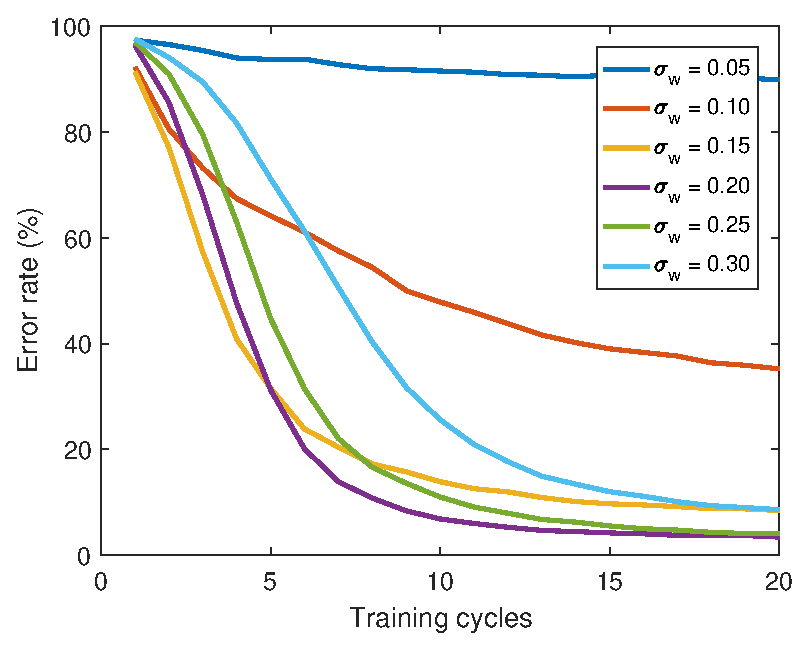
\includegraphics[width=\textwidth]{figs/w0_hlms.eps}
		\caption{HLMS}
	\end{subfigure}%

	\begin{subfigure}[h!]{0.75\textwidth}
		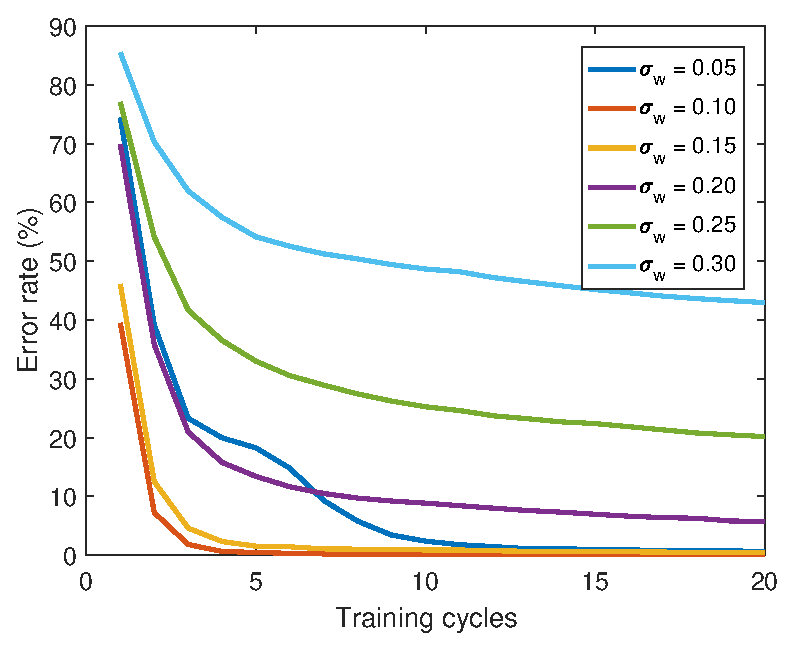
\includegraphics[width=\textwidth]{w0_bp.eps}
		\caption{Backpropagation}
	\end{subfigure}
	\caption{Classification error on the test set for several values of $\sigma_w$ for (a) HLMS and (b) backpropagation. In this experiment, $\rho = 75\%$. All other parameters are as listed in Table~\ref{tab:param}.} \label{fig:w0}
\end{figure}
\FloatBarrier

Fig.~\ref{fig:w02} shows the same experiment of Fig.~\ref{fig:w0}, but now the number of hidden layer neurons was doubled to 300. 

Fig.~\ref{fig:w02}a shows that increasing the number of hidden layer neurons reduced the steady-state error of HLMS. For this new network with 300 neurons in each hidden layer, best performance was achieved when $\sigma_w = 0.15$, differently from before.

Following equation \eqref{eq:w0}, backprop must have $\sigma_w = 1/\sqrt{300} = 0.0577$ to achieve good performance. This is verified in Fig.~\ref{fig:w02}b. Small error is also achieved when $\sigma_w = 0.1$, but larger values of $\sigma_w$ can lead to significantly worse performance.

\FloatBarrier
\begin{figure}[h!]
	\centering
	\begin{subfigure}[h!]{0.75\textwidth}
		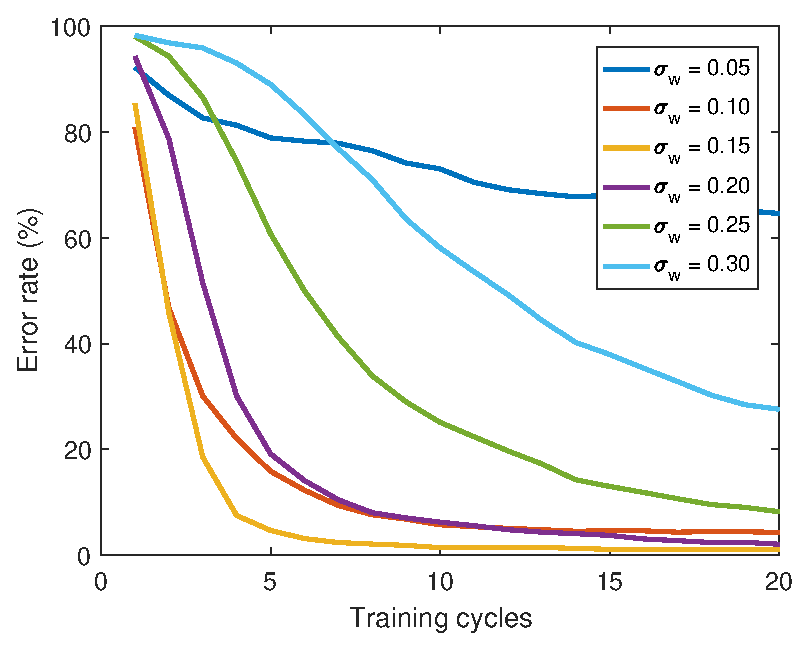
\includegraphics[width=\textwidth]{figs/w0_hlms_300.eps}
		\caption{HLMS}
	\end{subfigure}%
	
	\begin{subfigure}[h!]{0.75\textwidth}
		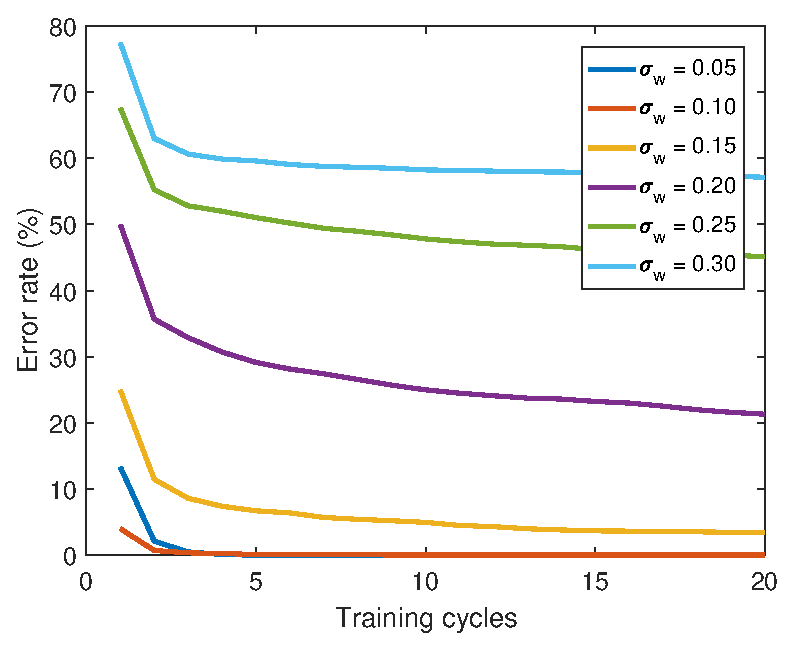
\includegraphics[width=\textwidth]{w0_bp_300.eps}
		\caption{Backpropagation}
	\end{subfigure}
	\caption{Classification error on the test set for several values of $\sigma_w$ for (a) HLMS and (b) backpropagation. In this experiment, $\rho = 75\%$, and the number of hidden layer neurons was 300. All other parameters are as listed in Table~\ref{tab:param}. } \label{fig:w02}
\end{figure}
\FloatBarrier

\subsection*{Effect of $\mu$}

This experiment explores the dependency of HLMS and backprop on the adaptation rate $\mu$. Learning curves for several values of $\mu$ are shown in Fig.~\ref{fig:mu}. 

As expected, increasing $\mu$ leads to faster convergence, but it increases the steady-state error. The same behavior is also observed in the backprop algorihtm (Fig.~\ref{fig:mu}b). However, the steady-state error in that case is very small.


\FloatBarrier
\begin{figure}[b!]
	\centering
	\begin{subfigure}[h!]{0.72\textwidth}
		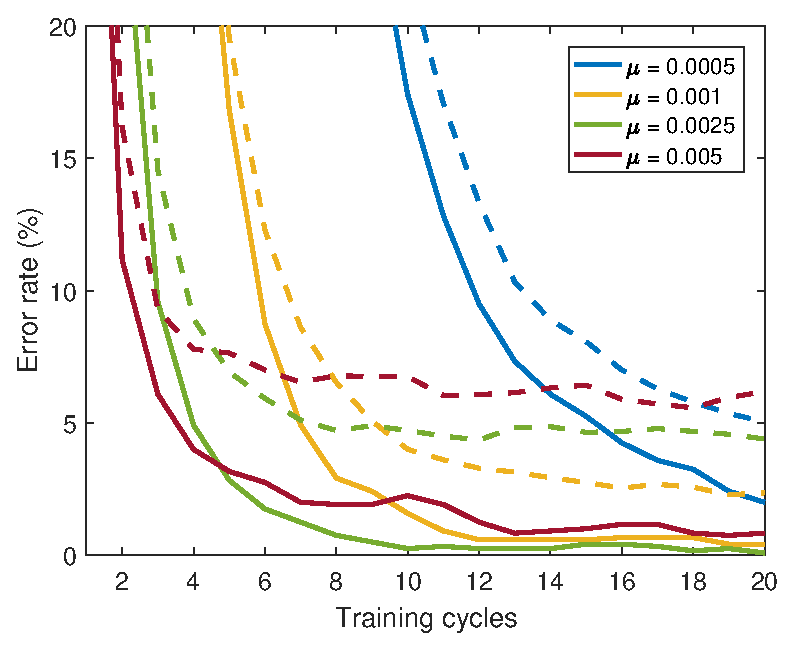
\includegraphics[width=\textwidth]{figs/mu_hlms.eps}
		\caption{HLMS}
	\end{subfigure}%
	
	\begin{subfigure}[h!]{0.72\textwidth}
		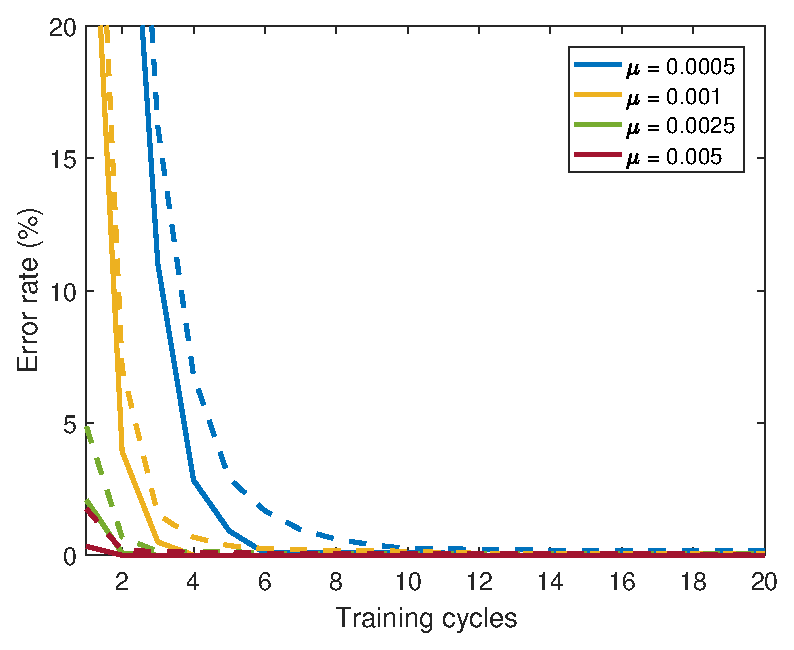
\includegraphics[width=\textwidth]{mu_bp.eps}
		\caption{Backpropagation}
	\end{subfigure}
	\caption{Learning curves for several values of $\mu$ for (a) HLMS and (b) backpropagation. $\rho = 75\%$. All other parameters are as listed in Table~\ref{tab:param}. Solid lines (\sampleline{}) represent training error, while dashed lines (\sampleline{dashed}) represent test error.} \label{fig:mu}
\end{figure}
\FloatBarrier

\subsection*{Effect of $\gamma$}

This experiment explores the dependency of HLMS on the parameter $\gamma$. Learning curves for several values of $\gamma$ are shown in Fig.~\ref{fig:gamma_hlms}. From Fig.~\ref{fig:gamma_hlms}, it seems that $\gamma = 0.3$ or $\gamma = 0.4$ offer the best trade-off between fast convergence and small steady-state error.

\FloatBarrier
\begin{figure}[h!]
	\centering
	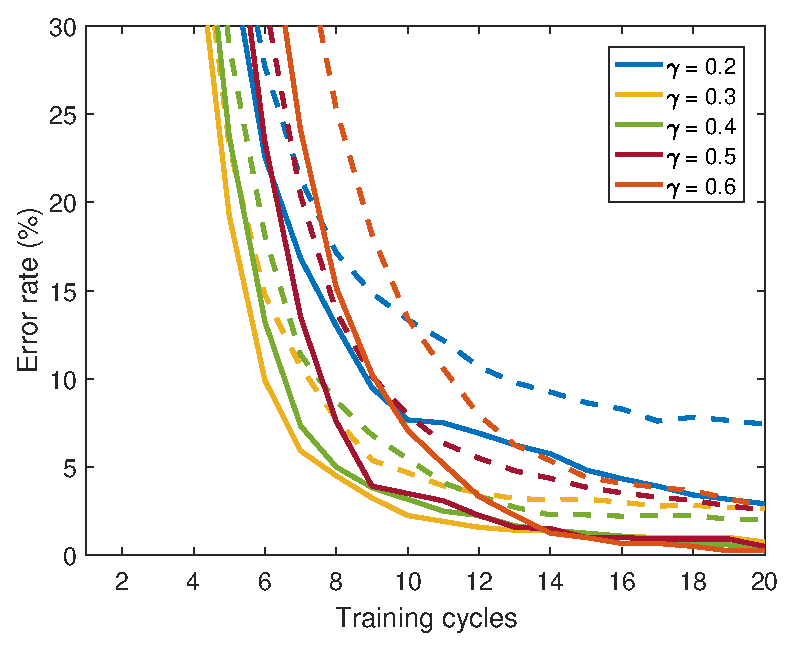
\includegraphics[scale=0.7]{figs/gamma_hlms.eps}
	\caption{Learning curves for several values of $\gamma$. In this experiment, $\rho = 75\%$. All other parameters are as listed in Table~\ref{tab:param}. Solid lines (\sampleline{}) correspond to training error, while dashed lines (\sampleline{dashed}) correspond to test error.}
	\label{fig:gamma_hlms}
\end{figure}
\FloatBarrier

\newpage
\subsection*{Effect of $\rho$}

When $\rho = 50\%$, HLMS and backprop achieve 0 \% error in the test set. For $\rho = 75\%$ the error in the test set is non-zero, but the error is smaller for backprop.

\FloatBarrier
\begin{figure}[b!]
	\centering
	\begin{subfigure}[h!]{0.75\textwidth}
		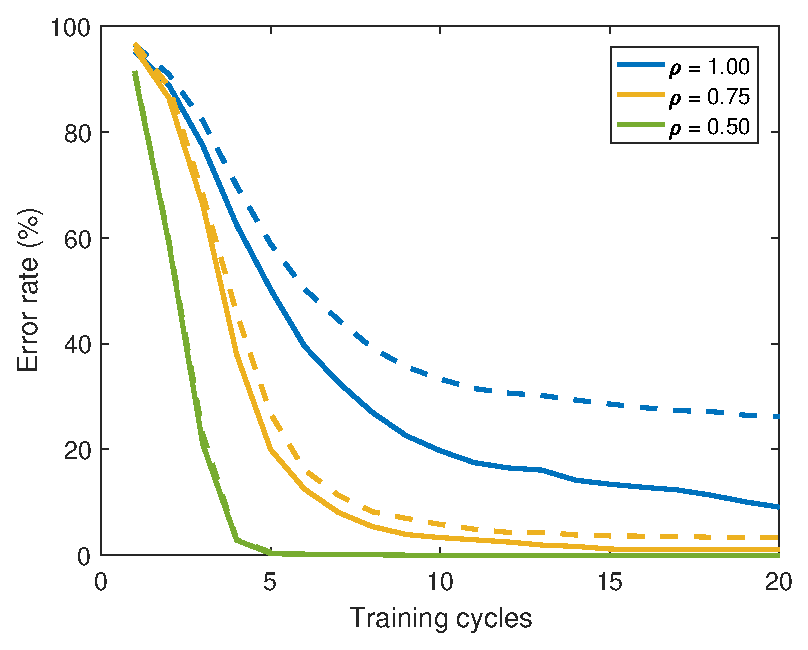
\includegraphics[width=\textwidth]{figs/rho_hlms.eps}
		\caption{HLMS}
	\end{subfigure}%
	
	\begin{subfigure}[h!]{0.75\textwidth}
		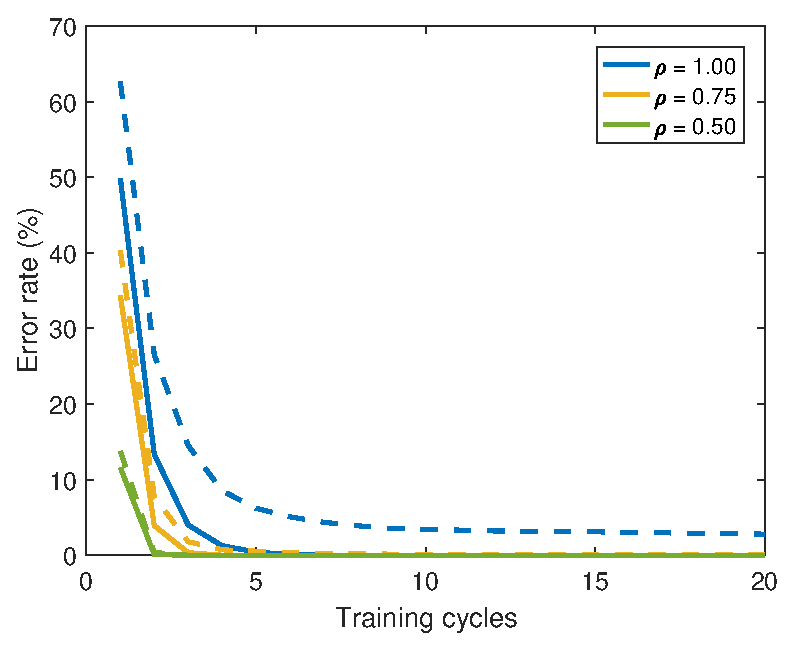
\includegraphics[width=\textwidth]{rho_bp.eps}
		\caption{Backpropagation}
	\end{subfigure}
	\caption{Learning curves for several values of $\rho$ for (a) HLMS and (b) backpropagation. All parameters are as listed in Table~\ref{tab:param}. Solid lines (\sampleline{}) correspond to training error, while dashed lines (\sampleline{dashed}) correspond to test error.} \label{fig:rho}
\end{figure}
\FloatBarrier

\end{document}